%# -*- coding: utf-8-unix -*-
%%==================================================
\tikzset{every picture/.style={line width=0.75pt}} %set default line width to 0.75pt    

\chapter{高中物理常用数据及图像}

\section{常用物理学常量}

\begin{table}[h]
\centering
\begin{threeparttable}
\begin{tabular}{|l|l|l|l|}
\hline
\textbf{符号} & \textbf{名称} & \textbf{精确值}\tnote{1} & \textbf{高中常用值}\\
\hline
$g$ & 重力加速度 & $9.80665 m/s^2$ & $10m/s^2$ \\
$G$ & 引力常量 & $6.67384 \times 10^{11} N \cdot m^2/kg^2$ & $6.67 \times 10^{-11} N \cdot m^2/kg^2$ \\
$e$ & 元电荷 & $1.602176565 \times 10^{-19} C$ & $1.6 \times 10^{-19} C$ \\ 
$k$ &  静电力常量 & $8987551788 N \cdot m^2 / C^2$ & $9 \times 10^{9} N \cdot m^2 /C^2$ \\
$c$ & 真空中光速 & $299792458 m/s$ & $3 \times 10^{8} m/s$ \\
$h$ & 普朗克常数 & $6.62606957 \times 10^{-34} J \cdot s$ & $6.63 \times 10^{-34} J \cdot s$ \\
\hline
\end{tabular}
\begin{tablenotes}
\item[1] 精确值参考了CODATA(2010)推荐值,可能跟高中课本有细微出入
\end{tablenotes}
\end{threeparttable}
\end{table}

\section{常用估计值}

\begin{center}
\begin{tabular}{|l|l|l|l|}
\hline
\textbf{符号} & \textbf{名称} & \textbf{估计值} & \textbf{备注} \\
\hline
$R_{earth}$ & 地球半径  & $6400 km$  & \\
$\rho_{earth}$ & 地球平均密度 & $5500 kg/m^3$ & 水密度的5.5倍 \\
$R_{sync}$ & 同步卫星轨道半径  & $42240km$ & 地球半径的$6.6$倍\\
$U_{m}$ & $220V$市电振幅 & $311 V$ & $311 \approx 220 \sqrt{2}$\\
\hline
\end{tabular}
\end{center}

\section{常用换算}

\subsection{词头换算}

\begin{center}
\begin{tabular}{|l|l|l||l|l|l|}
\hline
\textbf{名称} & \textbf{符号} & \textbf{数值} & \textbf{名称} & \textbf{符号} & \textbf{数值} \\
\hline
千 & $k$ & $1k=10^3$ & 兆 & $M$ & $1M = 10^6$ \\
毫 & $m$ & $1m=10^{-3}$ & 微 & $\mu$ & $1\mu = 10^{-6}$\\
纳 & $n$ & $1n=10^{-9}$ & 皮 & $p$ & $1p = 10^{-12}$\\
\hline
\end{tabular}
\end{center}

\subsection{单位换算}

\begin{table}[h]
\centering
\begin{threeparttable}
\begin{tabular}{|l|l||l|l|}
\hline
\textbf{单位}  & \textbf{数值关系} & \textbf{单位} & \textbf{数值关系} \tnote{1}\\
米每秒 $\to$ 千米每小时  & $1m/s = 3.6km/h$ & 千瓦时 $\to$ 焦耳 & $1kW \cdot h = 3.6 \times 10^{6} J$\\

\hline

\hline
\end{tabular}
\begin{tablenotes}
\item[1] 精确值参考了CODATA(2010)推荐值,可能跟高中课本有细微出入
\end{tablenotes}
\end{threeparttable}
\end{table}

\section{常用小量近似}
\label{s_xljs}

考虑到2022年全国甲卷压轴题需要使用小量近似,故在此给出高中中常见的小量近似(所有的小量近似表达式都是将函数做0处的泰勒(Taylor)展开,只保留前一阶项或者二阶项得来)

下面所有式子中,$x \ll 1$(即$x$为小量)

\begin{itemize}
\item $\sin x \approx \tan x \approx x$
\item $\cos x \approx 1 - \frac{x^2}{2}$
\item $(1+x)^n \approx 1 + nx$($n$为常数)
\item $ln(x+1) \approx x - \frac{x^2}{2}$
\item $e^x \approx 1 + x + \frac{x^2}{2}$
\end{itemize}

后三项不太常用,考试中若出现一般也会给,可以不记忆。

\section{常用物理图像}

\subsection{等量同种电荷}

下图中均取电荷$q=1C$,位于$(0.5m,0)$、$(-0.5m,0)$

\begin{figure}[H]
\begin{minipage}[b]{0.4\linewidth}
\centering
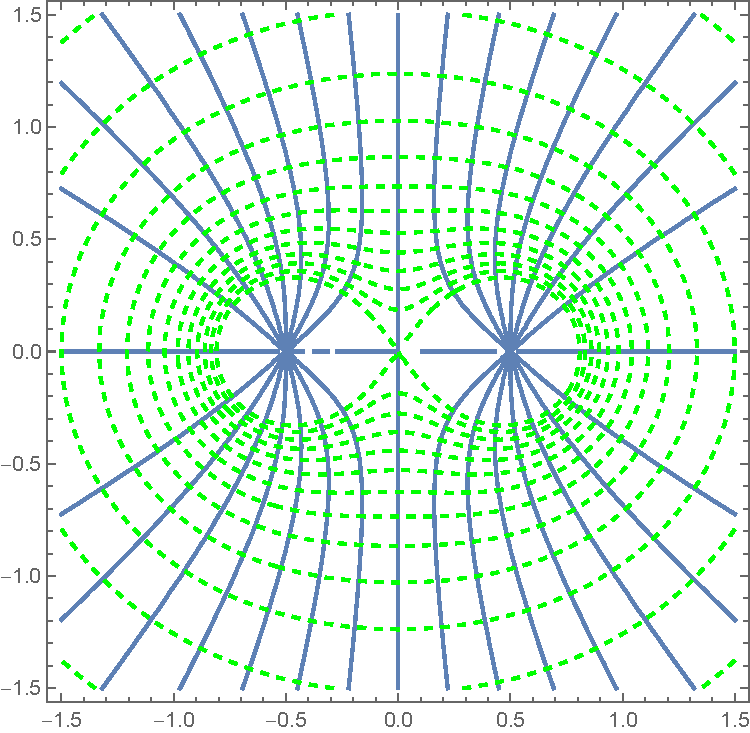
\includegraphics[width=\textwidth]{pic_data/T/dltzdh_p1.pdf}
\caption{电场线与等距等势面}
\end{minipage}
\hfill
\begin{minipage}[b]{0.4\linewidth}
\centering
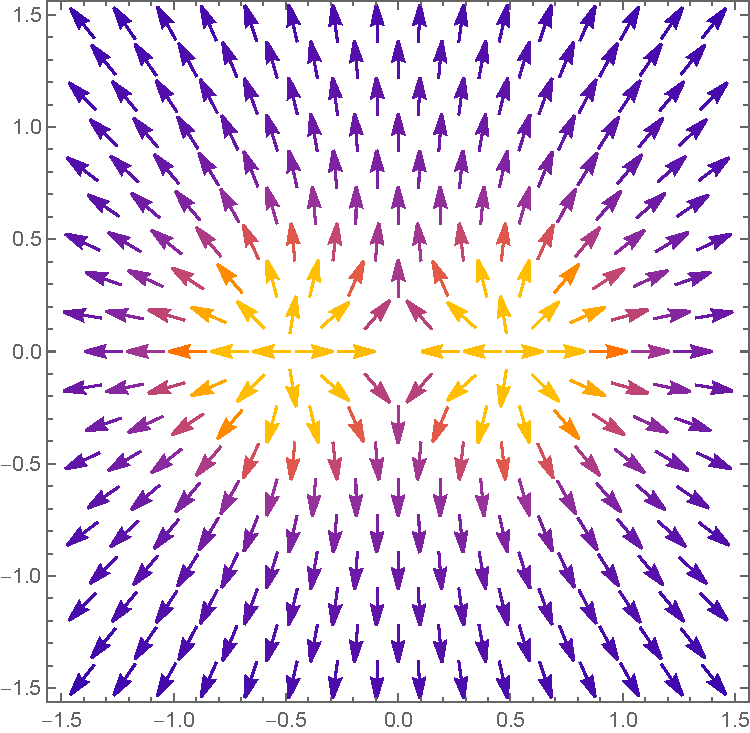
\includegraphics[width=\textwidth]{pic_data/T/dltzdh_p2.pdf}
\caption{电场场强与方向\protect \footnotemark}
\end{minipage}
\end{figure}
\footnotetext{箭头颜色表示场强,颜色越亮场强越大,下同}

\begin{figure}[H]
\begin{minipage}[b]{0.4\linewidth}
\centering
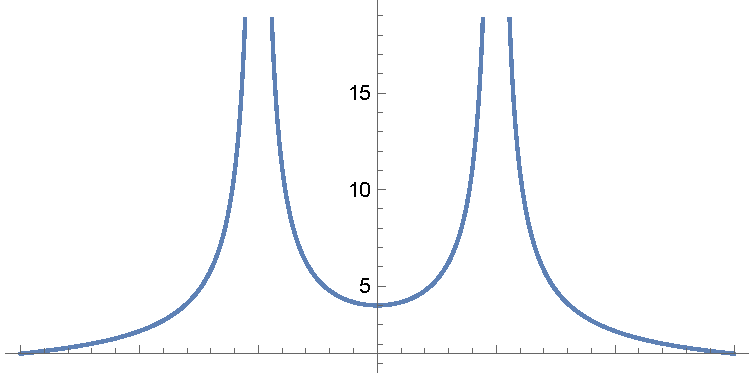
\includegraphics[width=\textwidth]{pic_data/T/phix.pdf}
\caption{沿$x$轴电势($\phi - x$图)}
\end{minipage}
\hfill
\begin{minipage}[b]{0.4\linewidth}
\centering
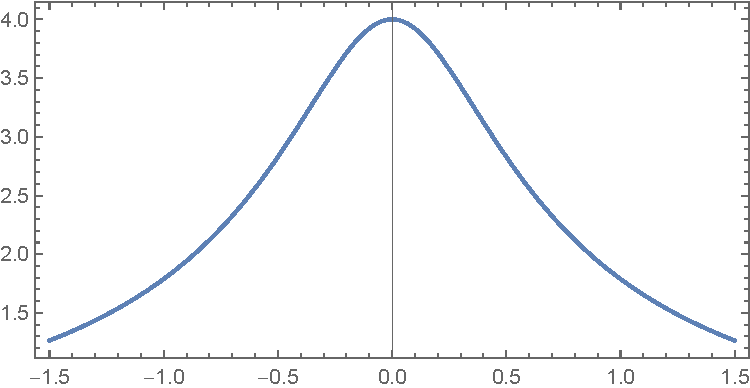
\includegraphics[width=\textwidth]{pic_data/T/phiy.pdf}
\caption{沿$y$轴电势($\phi - y$图)}
\end{minipage}
\end{figure}

\begin{figure}[H]
\begin{minipage}[b]{0.4\linewidth}
\centering
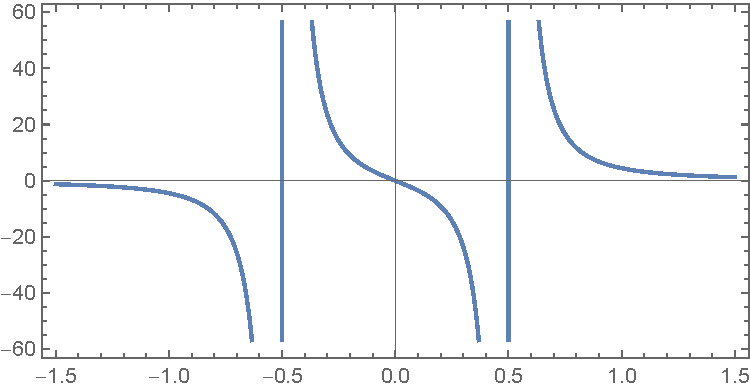
\includegraphics[width=\textwidth]{pic_data/T/Ex-x.pdf}
\caption{沿$x$轴$x$方向电场($E_x - x$图)}
\end{minipage}
\hfill
\begin{minipage}[b]{0.4\linewidth}
\centering
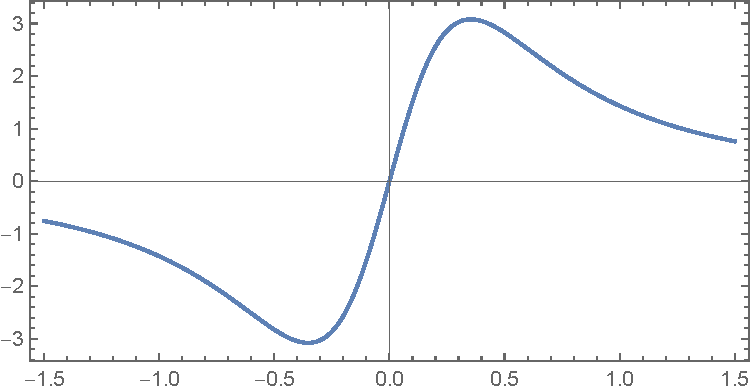
\includegraphics[width=\textwidth]{pic_data/T/Ey-y.pdf}
\caption{沿$y$轴$y$方向电场($E_y - y$图)}
\end{minipage}
\end{figure}

\subsection{等量异种电荷}

下图中取电荷$q=1C$,位于$(-0.5m,0)$;电荷$q=-1C$,位于$(0.5m,0)$

\begin{figure}[H]
\begin{minipage}[b]{0.4\linewidth}
\centering
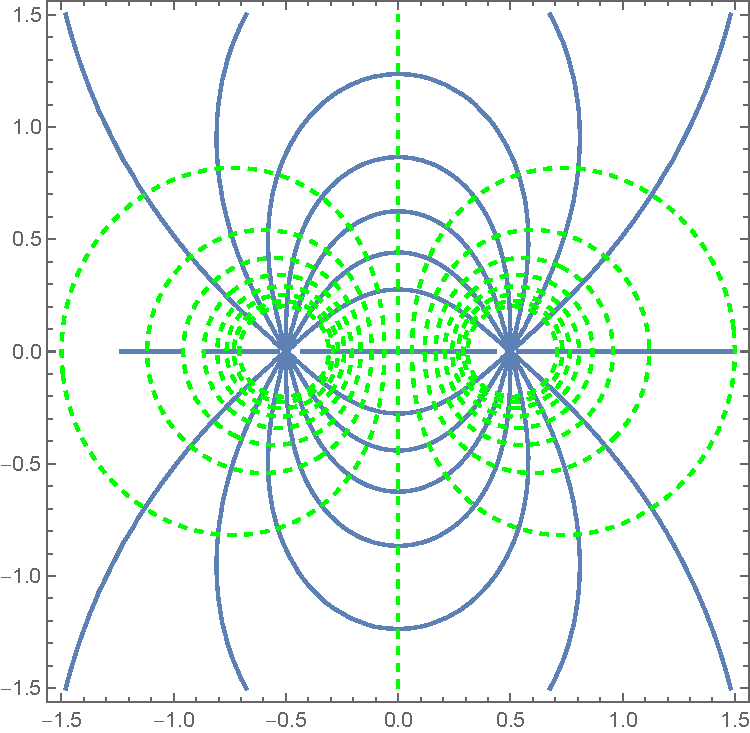
\includegraphics[width=\textwidth]{pic_data/Y/dlyzdh_p1.pdf}
\caption{电场线与等距等势面}
\end{minipage}
\hfill
\begin{minipage}[b]{0.4\linewidth}
\centering
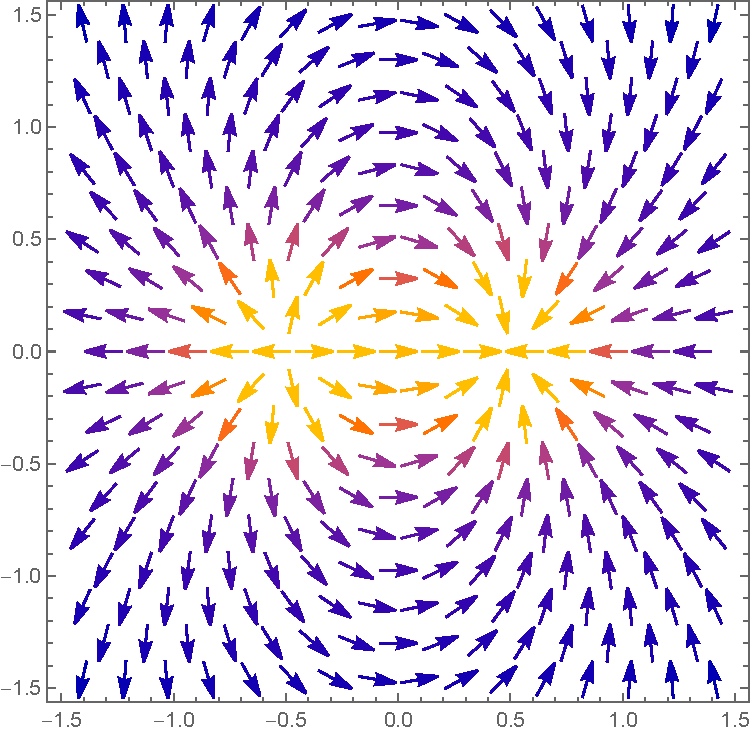
\includegraphics[width=\textwidth]{pic_data/Y/dlyzdh_p2.pdf}
\caption{电场场强与方向}
\end{minipage}
\end{figure}

\begin{figure}[H]
\begin{minipage}[b]{0.4\linewidth}
\centering
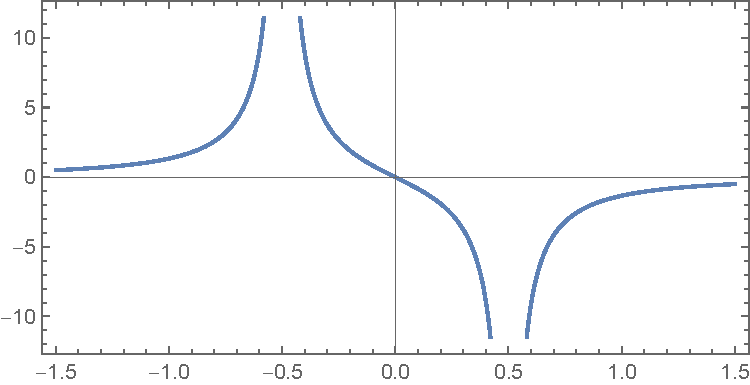
\includegraphics[width=\textwidth]{pic_data/Y/phix.pdf}
\caption{沿$x$轴电势($\phi - x$图)}
\end{minipage}
\hfill
\begin{minipage}[b]{0.4\linewidth}
\centering
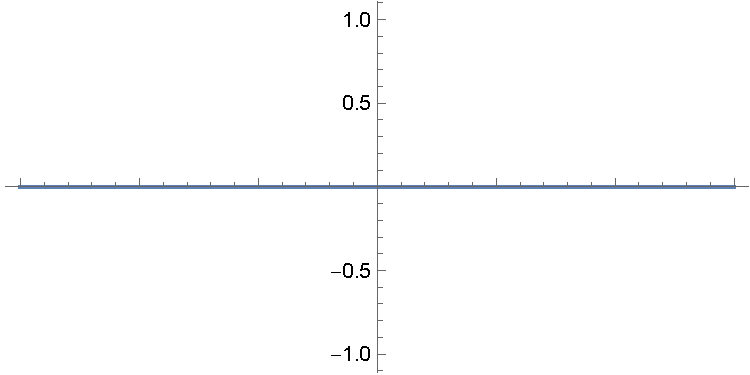
\includegraphics[width=\textwidth]{pic_data/Y/phiy.pdf}
\caption{沿$y$轴电势($\phi - y$图)}
\end{minipage}
\end{figure}

\begin{figure}[H]
\begin{minipage}[b]{0.4\linewidth}
\centering
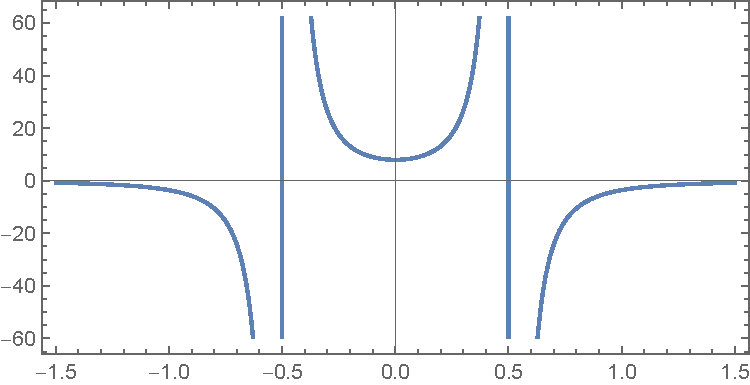
\includegraphics[width=\textwidth]{pic_data/Y/Ex-x.pdf}
\caption{沿$x$轴$x$方向电场($E_x - x$图)}
\end{minipage}
\hfill
\begin{minipage}[b]{0.4\linewidth}
\centering
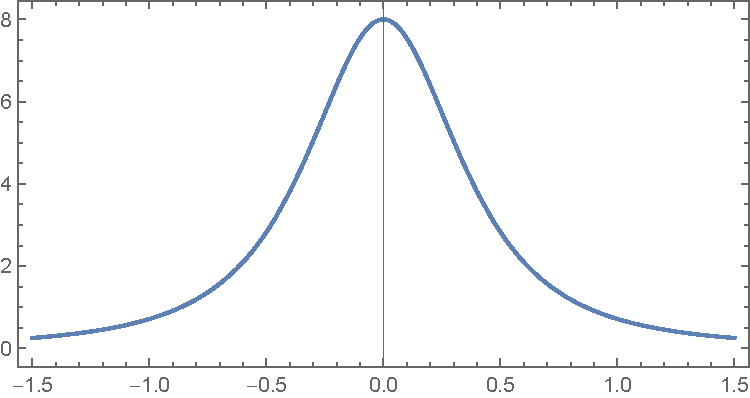
\includegraphics[width=\textwidth]{pic_data/Y/Ex-y.pdf}
\caption{沿$y$轴$x$方向电场($E_x - y$图)}
\end{minipage}
\end{figure}

\subsection{磁场}

\begin{figure}[H]
\begin{minipage}[b]{0.4\linewidth}
\centering
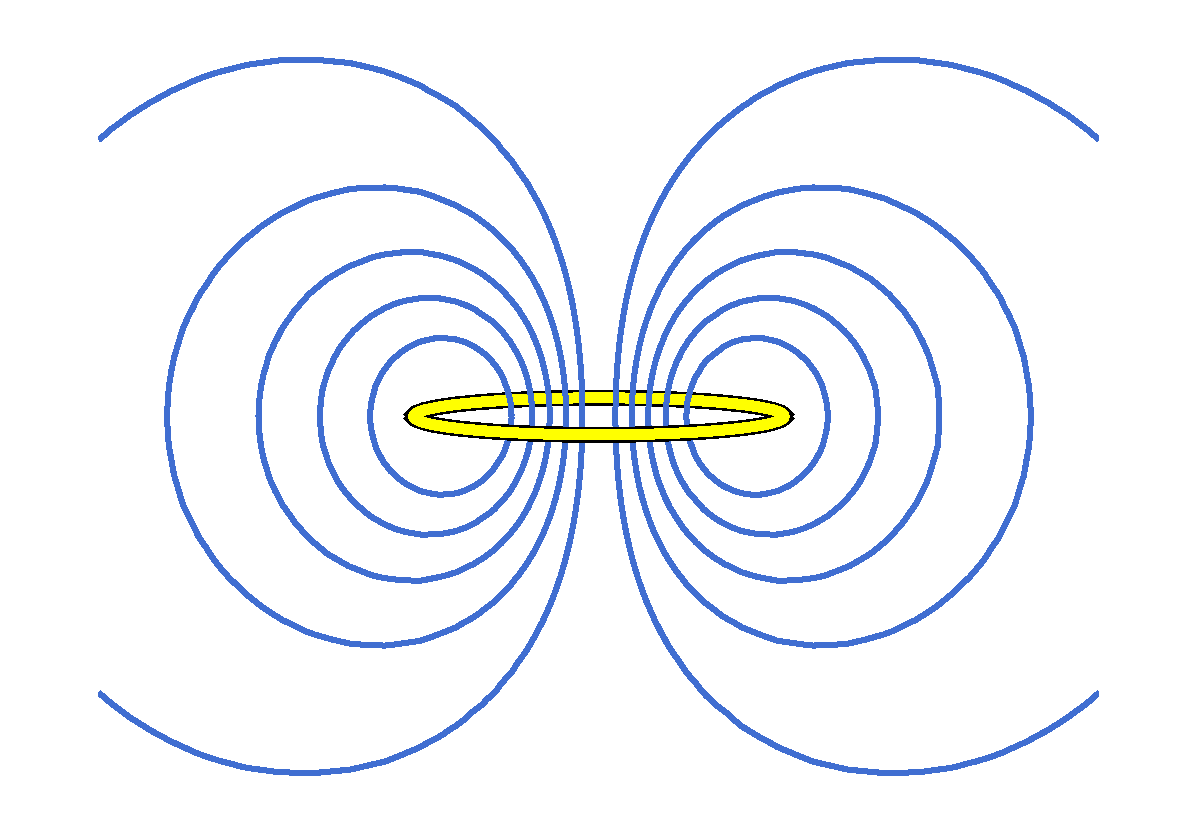
\includegraphics[width=\textwidth]{pic_data/dlhcc.pdf}
\stepcounter{footnote}
\caption{通电圆环磁场\protect \footnotemark[\value{footnote}]}
\end{minipage}
\hfill
\begin{minipage}[b]{0.4\linewidth}
\centering
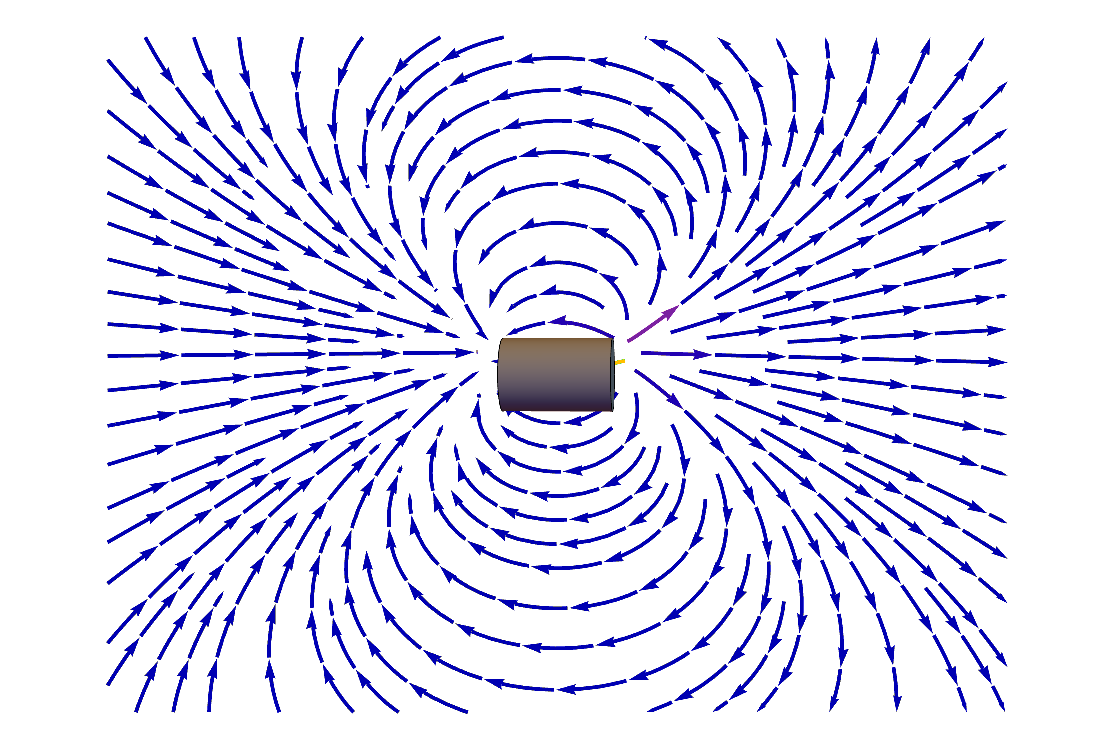
\includegraphics[width=\textwidth]{pic_data/txctcc.pdf}
\stepcounter{footnote}
\caption{条形磁铁磁场\protect \footnotemark[\value{footnote}]}
\end{minipage}
\end{figure}

\addtocounter{footnote}{-1}
\footnotetext[\value{footnote}]{图像原作者:S.M.Blinder 链接:\url{https://demonstrations.wolfram.com/MagneticFieldOfACurrentLoop/},通过CC BY-NC-SA协议共享}
\stepcounter{footnote}
\footnotetext[\value{footnote}]{图像原作者:S.M.Blinder 链接:\url{https://demonstrations.wolfram.com/MagneticFieldOfACylindricalBarMagnet/},通过CC BY-NC-SA协议共享}

%\subsection{}